\documentclass[a4paper,UTF8]{article}
\usepackage{xeCJK}

%\usepackage{ctex}
\usepackage[margin=1.25in]{geometry}
\usepackage{color}
\usepackage{graphicx}
\usepackage{amssymb}
\usepackage{amsmath}
\usepackage{amsthm}
\usepackage{enumerate}
\usepackage{bm}
\usepackage[colorlinks,
            linkcolor=red,
            anchorcolor=blue,
            citecolor=green]{hyperref}
\usepackage{epsfig}
\usepackage{color}
\usepackage{mdframed}
\usepackage{lipsum}
\usepackage{mathtools}
\usepackage{algorithm}
\usepackage{algorithmic}
\newmdtheoremenv{thm-box}{myThm}
\newmdtheoremenv{prop-box}{Proposition}
\newmdtheoremenv{def-box}{define}

\setlength{\evensidemargin}{.25in}
\setlength{\textwidth}{6in}
\setlength{\topmargin}{-0.5in}
\setlength{\topmargin}{-0.5in}
% \setlength{\textheight}{9.5in}
%%%%%%%%%%%%%%%%%%set header and footer here%%%%%%%%%%%%%%%%%%
\usepackage{fancyhdr}                                
\usepackage{lastpage}                                           
\usepackage{layout}                                             
\footskip = 10pt 
\pagestyle{fancy}                    
\lhead{2019, Spring}                    
\chead{Computer Vision: Representation and Recognition}
\rhead{Assignment 1}                                                                                               
\cfoot{\thepage}                                                
\renewcommand{\headrulewidth}{1pt}  			%header
\setlength{\skip\footins}{0.5cm}    			
\renewcommand{\footrulewidth}{0pt}  		

\makeatletter 							
\def\headrule{{\if@fancyplain\let\headrulewidth\plainheadrulewidth\fi%
\hrule\@height 1.0pt \@width\headwidth\vskip1pt	
\hrule\@height 0.5pt\@width\headwidth  			
\vskip-2\headrulewidth\vskip-1pt}      			
 \vspace{6mm}}     						
\makeatother  

%%%%%%%%%%%%%%%%%%%%%%%%%%%%%%%%%%%%%%%%%%%%%%
\numberwithin{equation}{section}
\newtheorem{myThm}{myThm}
\newtheorem*{myDef}{Definition}
\newtheorem*{mySol}{Solution}
\newtheorem*{myProof}{Proof}
\newcommand{\indep}{\rotatebox[origin=c]{90}{$\models$}}
\newcommand*\diff{\mathop{}\!\mathrm{d}}

\usepackage{multirow}
\renewcommand\refname{reference}








\linespread{1.3}
\setlength{\parskip}{12pt}
%%%%%%%%%%%%%%%%%%%%%%%%%%%%%%%%%%%%%%%%%%%%%%%%%%%%%%%%%%%%%%%%
\begin{document}
\title{Computer Vision: Representation and Recognition\\
Assignment 1}
\author{161180038, 广进, \href{mailto:guangjin1998@gmail.com}{guangjin1998@gmail.com}}
\maketitle

\section{Linear Filters (30 points)}
\subsection{question1(a)}
思路:使用卷积的 flip and shift 来解这道题更加直观,而不是用卷积公式来解:
\begin{description}
\item[step 1:]pad $I$ and flip $F$ (padding 过程中,$I$ 要上下各增加 $m-1=1$ 行,左右各增加 $n-1=1$ 行,其中 $F$ 的大小是 $m×n=2×2$):
\begin{equation}
I_{padding}={
\left[ \begin{array}{ccccc}
0 & 0 & 0 & 0 & 0\\
0 & 2 & 0 & 1 & 0\\
0 & 1 & -1 & 2 & 0\\
0 & 0 & 0 & 0 & 0
\end{array} 
\right ]},
F_{flip}={
\left[ \begin{array}{cc}
-1&1\\
-1&1
\end{array}
\right ]}
\end{equation}
\item[step 2:] $F_{flip}$ 在 $I_{padding}$上移动,对应位置相乘再整体求和:
示例如下:
\begin{equation}
I_{left\_top}={
\left[ \begin{array}{cc}
0 & 0 \\
0 & 2
\end{array} 
\right ]},
F_{flip}={
\left[ \begin{array}{cc}
-1&1\\
-1&1
\end{array}
\right ]},
\Rightarrow 0*(-1)+0*1+0*(-1)+2*1=2
\end{equation}
\item[step3:] 就这样$F_{flip}$一个一个向右移动得到第一行结果:
\begin{equation}
{
\left[ \begin{array}{cccc}
2&-2&1&-1
\end{array} 
\right ]}
\end{equation}
\item[step4:] 再把$F_{flip}$在$I_{padding}$向下移动一行再做,以此类推,直到所有完成,得到最终答案:
\begin{equation}
I*F={
\left[ \begin{array}{cccc}
2&-2&1&-1\\
3&-4&4&-3\\
1&-2&3&-2
\end{array}
\right ]}
\end{equation}
\end{description}




\subsection{question1(b)}
思路:类似于上一题的做法,采用 flip and shift 的计算方法
\begin{description}
\item[step 1:]pad $I$ and flip $F_1$(padding 过程中,$I$ 只要上下各增加 $1$ 行):
\begin{equation}
I_{padding}={
\left[ \begin{array}{ccc}
0 & 0 & 0\\
2 & 0 & 1\\
1 & -1 & 2\\
0 & 0 & 0
\end{array} 
\right ]},
F_{1\_flip}={
\left[ \begin{array}{c}
1\\
1
\end{array}
\right ]}
\end{equation}
\item[step 2:] $F_{1\_flip}$ 在 $I_{padding}$上移动,对应位置相乘再整体求和:
示例如下:
\begin{equation}
I_{left\_top}={
\left[ \begin{array}{c}
0 \\
2
\end{array} 
\right ]},
F_{1\_flip}={
\left[ \begin{array}{c}
1\\
1
\end{array}
\right ]},
\Rightarrow 0*1+2*1=2
\end{equation}
\item[step3:] 就这样$F_{1\_flip}$一个一个向右移动得到第一行结果:
\begin{equation}
{
\left[ \begin{array}{ccc}
2&0&1
\end{array} 
\right ]}
\end{equation}
\item[step4:] 再把$F_{1\_flip}$在$I_{padding}$向下移动一行再做,以此类推,直到所有完成,得到最终答案:
\begin{equation}
I*F_1={
\left[ \begin{array}{cccc}
2&0&1\\
3&-1&3\\
1&-1&2
\end{array}
\right ]}
\end{equation}
\end{description}
下面计算 $(I*F_1)*F_2$:
\begin{description}
\item[step 1:]pad $(I*F_1)$ and flip $F_2$(padding 过程中,$(I*F_1)$ 只要左右各增加 $1$ 列):
\begin{equation}
(I*F_1)_{padding}={
\left[ \begin{array}{ccccc}
0&2&0&1&0\\
0&3&-1&3&0\\
0&1&-1&2&0
\end{array}
\right ]},
F_{2\_flip}={
\left[ \begin{array}{cc}
-1&1
\end{array}
\right ]}
\end{equation}
\item[step 2:] $F_{2\_flip}$ 在 $(I*F_1)_{padding}$上移动,对应位置相乘再整体求和:
示例如下:
\begin{equation}
(I*F_1)_{left\_top}={
\left[ \begin{array}{cc}
0&2
\end{array} 
\right ]},
F_{2\_flip}={
\left[ \begin{array}{cc}
-1&1
\end{array}
\right ]},
\Rightarrow 0*(-1)+2*1=2
\end{equation}
\item[step3:] 就这样$F_{2\_flip}$一个一个向右移动得到第一行结果:
\begin{equation}
{
\left[ \begin{array}{cccc}
2&-2&1&-1
\end{array} 
\right ]}
\end{equation}
\item[step4:] 再把$F_{2\_flip}$在$(I*F_1)_{padding}$向下移动一行再做,以此类推,直到所有完成,得到最终答案:
\begin{equation}
(I*F_1)*F_2={
\left[ \begin{array}{cccc}
2&-2&1&-1\\
3&-4&4&-3\\
1&-2&3&-2
\end{array}
\right ]}
\end{equation}
\end{description}
\subsection{question1(c)}
思路:将左右都套卷积公式展开
\begin{description}
\item[左式:]$$(I*F)[i,j]=\sum_{k,l}I[i-k,j-l]F[k,l]$$
\item[右式:]$$(I*F_1)[i,j]=\sum_{k}I[i-k,j]F_1[k,0]$$
\begin{align*}
((I*F_1)*F_2)[i,j]&=\sum_{l}(I*F_1)[i,j-l]F_2[0,l]\\
&=\sum_{l}(\sum_{k}I[i-k,j-l]F_1[k,0])F_2[0,l]\\
&=\sum_{l}(\sum_{k}I[i-k,j-l]F_1[k,0]F_2[0,l])\\
&=\sum_{k,l}I[i-k,j-l](F_1[k,0]F_2[0,l]))\\
&=\sum_{k,l}I[i-k,j-l]F[k,l]\\
&=(I*F)[i,j]
\end{align*}
\end{description}
证毕
\subsection{question1(d)}
思路:首先推出一个对于计算 flip and shift 乘法数目的一般性结论,再带入解决以下小问。
\newtheorem{thm}{Theorem}
\begin{thm}
\label{T:major}
对于 $I_{a×b}$ $F_{m×n}$,如果要 flip and shift $F$,一共会做$[(a+m-1)×(b+n-1)]×(m×n)$次乘法运算。
\end{thm}
\begin{proof}
对于 $I_{a×b}$ $F_{m×n}$,如果要 flip and shift $F$,则 $I$ 需要 pad:$I$ 上下各增加 $m-1$ 行,左右各增加 $n-1$ 列,进而 $I_{padding}$ 的大小为 $(a+(m-1)×2)×(b+(n-1)×2)$。所以,$F$ 每行会滑动 $(a+(m-1)×2)-(m-1)=a+m-1$ 次,每列会滑动 $(b+(n-1)×2)-(n-1)=b+n-1$ 次,一共会做 $(a+m-1)×(b+n-1)$ 个框的运算。而每个框大小为 $F$ 的大小,会做 $m×n$ 次乘法,所以一共会做$[(a+m-1)×(b+n-1)]×(m×n)$次乘法运算。
\end{proof}
\begin{enumerate}[(\romannumeral1)]
	\item 如果 flip and shift $I$,应用 Theorem~\ref{T:major},需要做$[(2+2-1)×(3+2-1)]×(2×3)=12×6=72$次乘法运算。
	\item 不相同。因为如果 flip and shift $F$,应用 Theorem~\ref{T:major},需要做$[(2+2-1)×(3+2-1)]×(2×2)=12×4=48$次乘法运算。
	\item 对于 part(b),$(I*F_1)$ 我们选择乘法运算次数更少的,即 flip and shift $F_1$,应用 Theorem~\ref{T:major},需要做$[(2+2-1)×(3+1-1)]×(2×1)=9×2=18$次乘法运算;$(I*F_1)*F_2$ 我们选择乘法运算次数更少的,即 flip and shift $F_2$,应用 Theorem~\ref{T:major},需要做$[(3+1-1)×(3+2-1)]×(1×2)=12×2=24$次乘法运算。一共要做$18+24=42$次乘法运算。
	\item 由于 $42<48$,method (b) 需要更少的计算次数。
\end{enumerate} 
\subsection{question1(e)}
\begin{enumerate}[(\romannumeral1)]
	\item 一般 image 比 filter 大,所以我们选择乘法次数少的,即 flip and shift $F$,应用 Theorem~\ref{T:major},需要做$[(M_1+M_2-1)×(N_1+N_2-1)]×(M_2×N_2)$次乘法运算;而 flip and shift $I$,应用 Theorem~\ref{T:major},需要做$[(M_1+M_2-1)×(N_1+N_2-1)]×(M_2×N_2)$次乘法运算。
	\item 设 $F=F_1F_2,where F_1:M_2×1 and F_2:1×N_2$,我们选择乘法次数少的,即 flip and shift $F_1$ 和 $F_2$。首先计算 $(I*F_1)$ 应用 Theorem~\ref{T:major},需要做$[(M_1+M_2-1)×(N_1+1-1)]×(M_2×1)=(M_1+M_2-1)×N_1×M_2$次乘法运算,得到$(I*F_1)大小:[M_1+M_2-1]×N_1$(见Theorem~\ref{T:major}的证明,最后的框数)。然后计算 $(I*F_1)*F_2$ 应用 Theorem~\ref{T:major},需要做$[([M_1+M_2-1]+1-1)×(N_1+N_2-1)]×(1×N_2)=(M_1+M_2-1)×(N_1+N_2-1)×N_2$次乘法运算。所以一共需要$(M_1+M_2-1)×N_1×M_2+(M_1+M_2-1)×(N_1+N_2-1)×N_2=(M_1+M_2-1)×[N_1×(M_2+N_2)+(N_2-1)×N_2]$
	\item 对于直接2D卷积:
	\begin{align*}
	&[(M_1+M_2-1)×(N_1+N_2-1)]×(M_2×N_2)\\
	&=O((M_1+M_2)(N_1+N_2)M_2N_2\\
	&=O(M_1N_1M_2N_2+M_1M_2N_2^2+M_2^2N_1N_2+M_2^2N_2^2)
	\end{align*}
	两次连续1D卷积:
	\begin{align*}
	&(M_1+M_2-1)×[N_1×(M_2+N_2)+(N_2-1)×N_2]\\
	&=O((M_1+M_2)×[N_1×(M_2+N_2)+N_2^2])\\
	&=O(M_1M_2N_1+M_2^2N_1+M_1N_1N_2+M_2N_1N_2+M_1N_2^2+M_2N_2^2)
	\end{align*}	
	由于
	\begin{align*}
	&O(M_1M_2N_1+M_1N_1N_2+M_2N_1N_2)=O(M_1N_1M_2N_2)\\
	&O(M_2^2N_1)=O(M_2^2N_1N_2)\quad O(M_1N_2^2+M_2N_2^2)=O(M_1M_2N_2^2)
	\end{align*}
	所以两次连续1D卷积更有效率:
	\begin{align*}
	&O(M_1M_2N_1+M_2^2N_1+M_1N_1N_2+M_2N_1N_2+M_1N_2^2+M_2N_2^2)\\
	&=O(M_1N_1M_2N_2+M_1M_2N_2^2+M_2^2N_1N_2+M_2^2N_2^2)
	\end{align*}
\end{enumerate} 



















\section{Question 2}
观看效果,采用如下滤波器:
\begin{equation}
h_0={
\left[ \begin{array}{ccc}
0.0625 & 0.125 & 0.0625\\
  0.125 & 0.25 & 0.125\\
  0.0625 & 0.125 & 0.0625
\end{array} 
\right ]},
h_1={
\left[ \begin{array}{ccccc}
-1&-2&0&2&1\\
-2&-4&0&4&2\\
-1&-2&0&2&1
\end{array} 
\right ]},
h_2={
\left[ \begin{array}{ccc}
-1 & -2 & -1\\
  -2 & -4 & -2\\
  0 & 0 & 0\\
  2 & 4 & 2\\
  1 & 2 & 1
\end{array} 
\right ]}
\end{equation}
效果如下:
\begin{figure}[htbp]
\centering
\begin{minipage}[t]{0.48\textwidth}
\centering
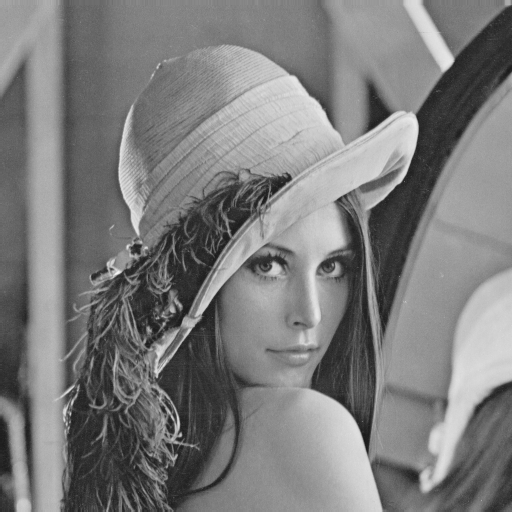
\includegraphics[width=6cm]{Lenna_gray.png}
\caption{Lenna 灰度图}
\end{minipage}
\begin{minipage}[t]{0.48\textwidth}
\centering
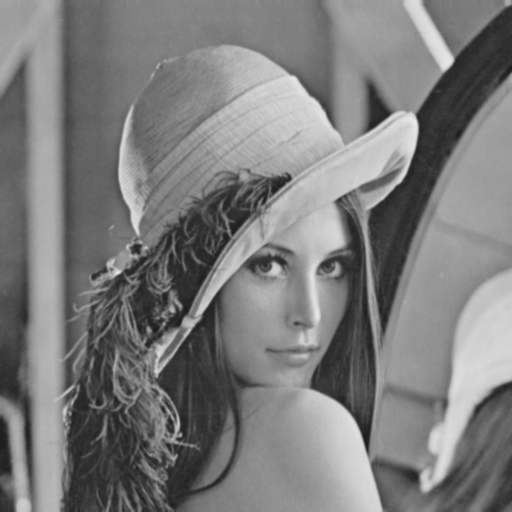
\includegraphics[width=6cm]{Lenna_filter_gauss.png}
\caption{经过高斯滤波器$h_0$卷积的效果}
\end{minipage}
\end{figure}
\begin{figure}[htbp]
\centering
\begin{minipage}[t]{0.48\textwidth}
\centering
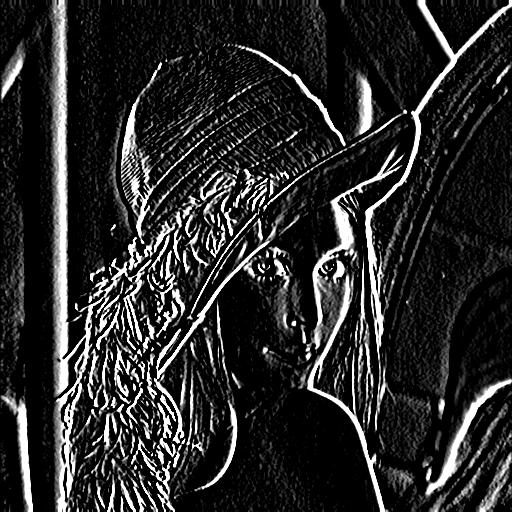
\includegraphics[width=6cm]{Lenna_filter.png}
\caption{经过滤波器$h_1$卷积的效果}
\end{minipage}
\begin{minipage}[t]{0.48\textwidth}
\centering
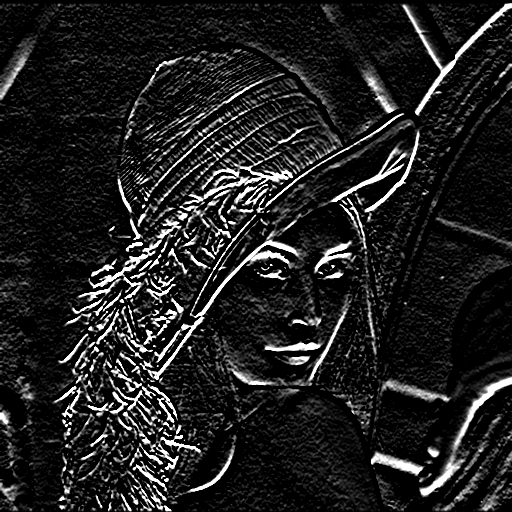
\includegraphics[width=6cm]{Lenna_filter_v.png}
\caption{经过滤波器$h_2$卷积的效果}
\end{minipage}
\end{figure}

























\section{Question 3}
\subsection{Global Histogram Equalization (三张图片示例)}
\subsubsection{Lenna 图片}
\begin{enumerate}[(\romannumeral1)]
	\item 转化为灰度图,采用书上(2.112)转换公式:$Y_{601}=0.299R+0.587G+0.114B$。转化后见图~\ref{Lenna:gray} :
	\item 原图的直方图见图~\ref{Lenna:count} ,累积分布函数见图~\ref{Lenna:cdf}  ,compensation transfer function 为 $f(I)=\alpha×c(I)+(1-\alpha)×I$(局部补偿,见课本公式(3.9)后面),最终直方图均衡化($f(I)=c(I),即\alpha=1$)结果见图~\ref{Lenna:processed},其直方图和累积分布函数分别见图~\ref{Lenna:Pcount} 和图~\ref{Lenna:Pcdf} 。图~\ref{Lenna:75p} 图~\ref{Lenna:50p} 和图~\ref{Lenna:25p} 分别是$\alpha$分别为0.75, 0.5, 0.25的图片。
\begin{figure}[htbp]
\centering
\begin{minipage}[t]{0.30\textwidth}
\centering
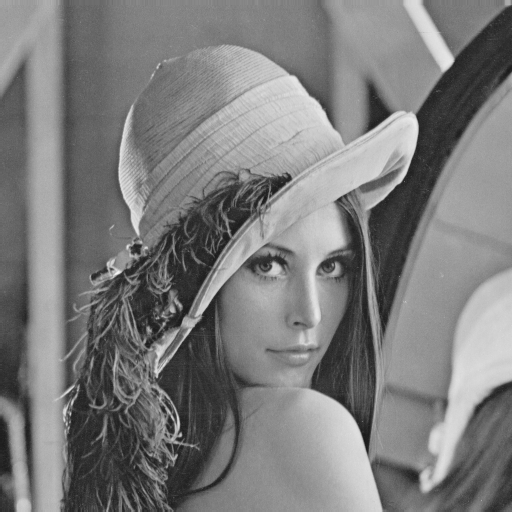
\includegraphics[width=4cm]{Lenna_gray.png}
\caption{Lenna 灰度图}
\label{Lenna:gray}
\end{minipage}
\centering
\begin{minipage}[t]{0.3\textwidth}
\centering
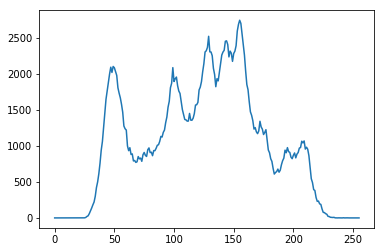
\includegraphics[width=1.0\textwidth]{global_pdf.png}
\caption{Lenna 直方图}
\label{Lenna:count}
\end{minipage}
\begin{minipage}[t]{0.3\textwidth}
\centering
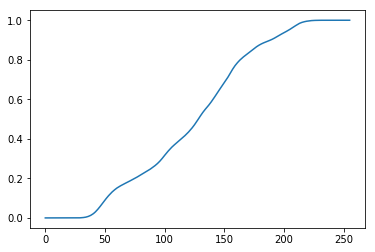
\includegraphics[width=1.0\textwidth]{global_cdf.png}
\caption{累积分布函数}
\label{Lenna:cdf}
\end{minipage}
\centering
\begin{minipage}[t]{0.30\textwidth}
\centering
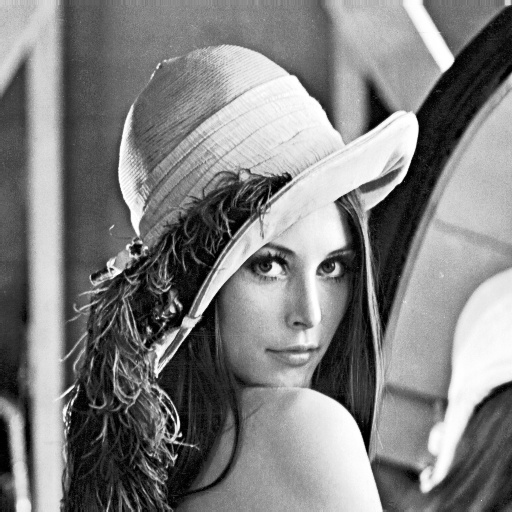
\includegraphics[width=4cm]{Lenna_processed.jpg}
\caption{Lenna $\alpha=1.00$}
\label{Lenna:processed}
\end{minipage}
\centering
\begin{minipage}[t]{0.3\textwidth}
\centering
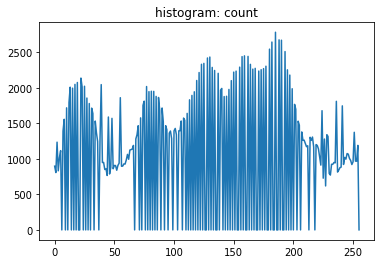
\includegraphics[width=1.0\textwidth]{Lenna_processed_count.png}
\caption{Lenna 直方图}
\label{Lenna:Pcount}
\end{minipage}
\begin{minipage}[t]{0.3\textwidth}
\centering
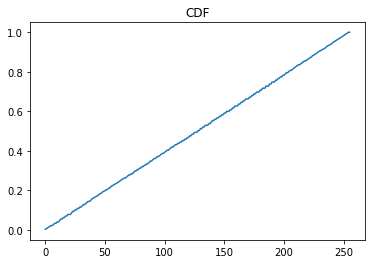
\includegraphics[width=1.0\textwidth]{Lenna_processed_cdf.png}
\caption{累积分布函数}
\label{Lenna:Pcdf}
\end{minipage}
\begin{minipage}[t]{0.3\textwidth}
\centering
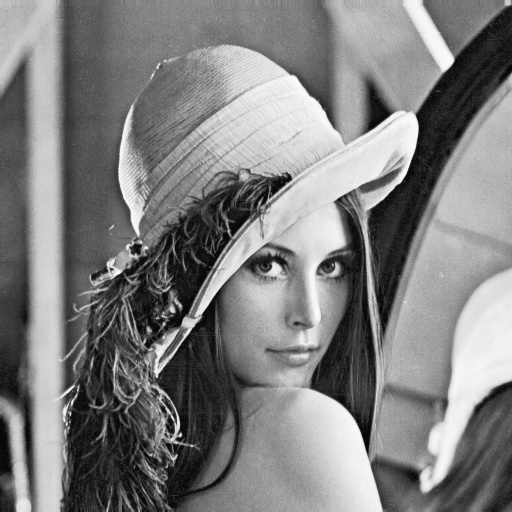
\includegraphics[width=4cm]{Lenna_processed_75.jpg}
\caption{ $\alpha=0.75$}
\label{Lenna:75p}
\end{minipage}
\begin{minipage}[t]{0.3\textwidth}
\centering
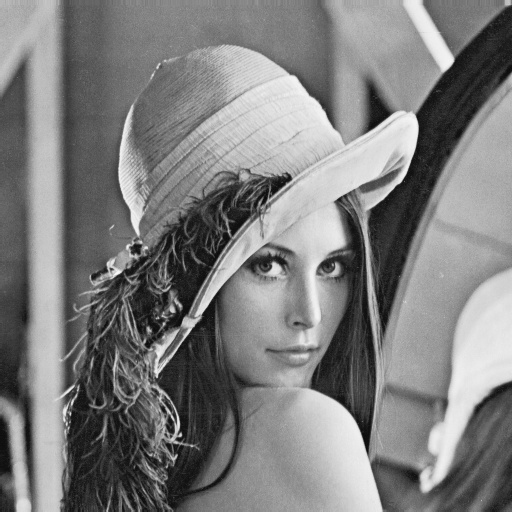
\includegraphics[width=4cm]{Lenna_processed_50.jpg}
\caption{  $\alpha=0.50$}
\label{Lenna:50p}
\end{minipage}
\begin{minipage}[t]{0.3\textwidth}
\centering
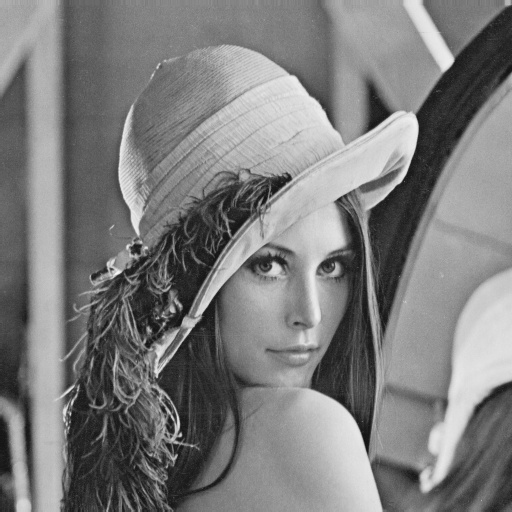
\includegraphics[width=4cm]{Lenna_processed_25.jpg}
\caption{ $\alpha=0.25$}
\label{Lenna:25p}
\end{minipage}
\end{figure}

	\item punch: 一般化,假如 pixel 前 $a\%$ 的变为纯白,pixel 后 $b\%$ 的变为纯黑,则有:\begin{equation}
compensation\ transfer\ function\ f(I)= {
\left\lbrace \begin{array}{ll}
0&if{\ } c(I) < b\%\\
\dfrac{c(I)-b\%}{1-a\%-b\%}&if {\ }b\% < c(I) < 1-a\% \\
1&if{\ } c(I) > 1-a\%
\end{array} 
\right. }
\end{equation}
punch 纯黑纯白各$5\%, 25\%, 40\%$分别见图~\ref{Lenna:5_punch} 、图~\ref{Lenna:25_punch} 和图~\ref{Lenna:40_punch} 。

\begin{figure}[htbp]
\centering
\begin{minipage}[t]{0.30\textwidth}
\centering
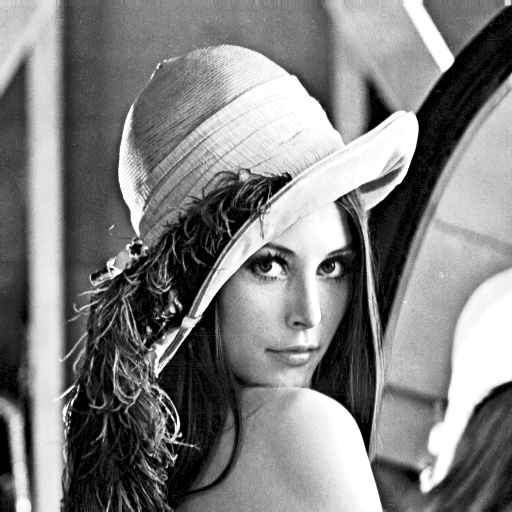
\includegraphics[width=4cm]{Lenna_punch_5_5.png}
\caption{ punch 5\% - 95\%}
\label{Lenna:5_punch}
\end{minipage}
\centering
\begin{minipage}[t]{0.30\textwidth}
\centering
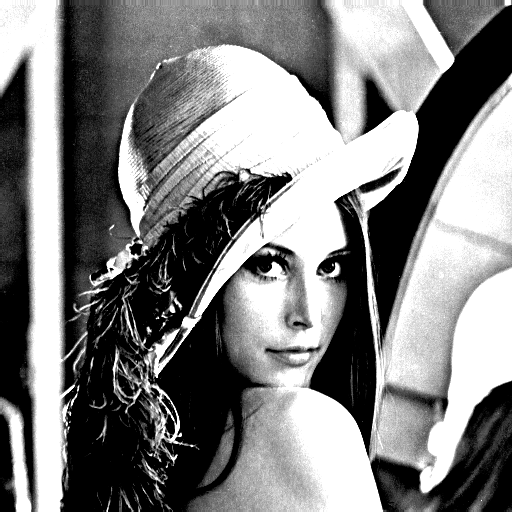
\includegraphics[width=4cm]{Lenna_punch_25_25.png}
\caption{ punch 25\% - 75\%}
\label{Lenna:25_punch}
\end{minipage}\centering 
\begin{minipage}[t]{0.30\textwidth}
\centering
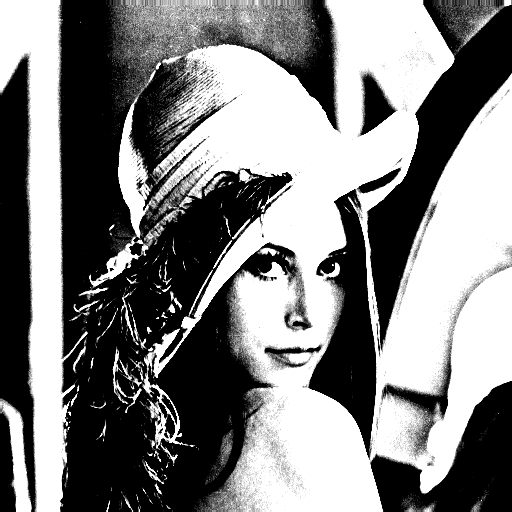
\includegraphics[width=4cm]{Lenna_punch_40_40.png}
\caption{ punch 40\% - 60\%}
\label{Lenna:40_punch}
\end{minipage}
\end{figure}

	\item limit local gain 就是要限制 transfer function $F(I) = cdf[I] < \lambda I$,也就是限制其倒数 $f'(x)<\lambda $。由于cdf是离散的,倒数用差分代替,而由于公式(3.9),cdf的差分便是$\dfrac{1}{N}h(I)$,再将截去的那些$h(I)$平均分布在每个$I$上。 分别将$N×\lambda $ 限制在10, 100, 1000,对于Lenna区别不是很大,见下图:
\begin{figure}[htbp]
\centering
\begin{minipage}[t]{0.30\textwidth}
\centering
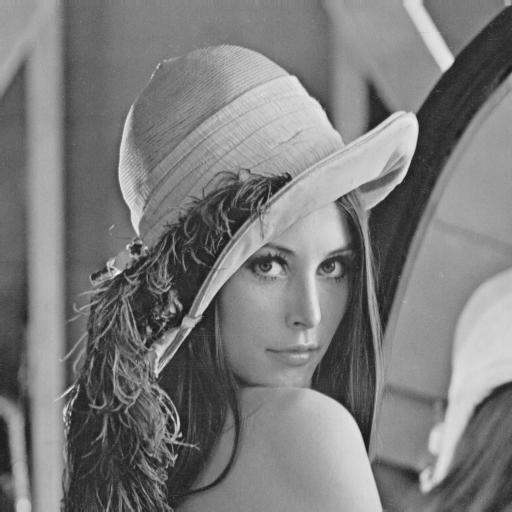
\includegraphics[width=4cm]{Lenna_limit_10.png}
\caption{$\lambda=10$}
\label{Lenna:10_lambda}
\end{minipage}
\centering
\begin{minipage}[t]{0.30\textwidth}
\centering
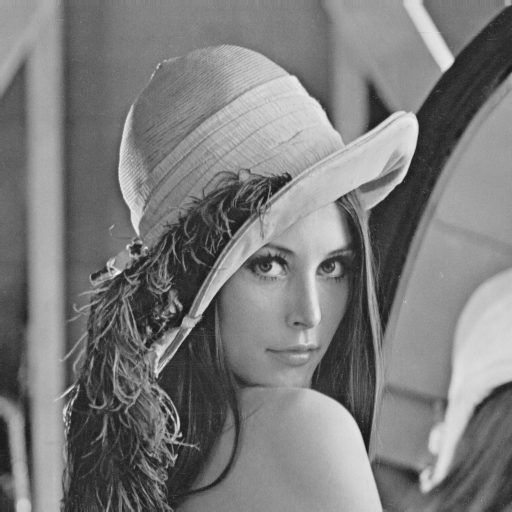
\includegraphics[width=4cm]{Lenna_limit_100.png}
\caption{$\lambda=100$}
\label{Lenna:100_lambda}
\end{minipage}
\centering
\begin{minipage}[t]{0.30\textwidth}
\centering
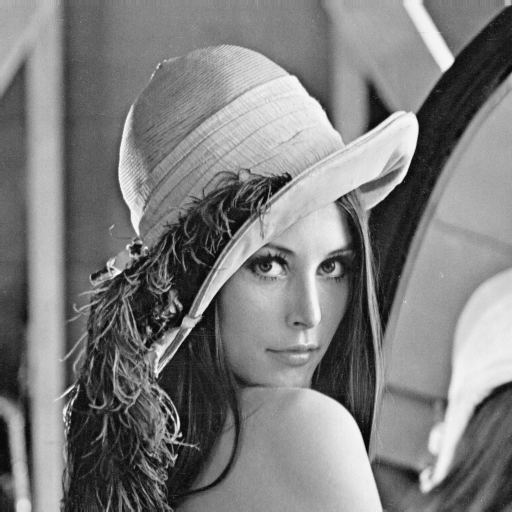
\includegraphics[width=4cm]{Lenna_limit_1000.png}
\caption{$\lambda=1000$}
\label{Lenna:1000_lambda}
\end{minipage}
\end{figure}
	\item gray image to color 方法如下:由书上公式(2.116),$r=\dfrac{R}{R+G+B}$ ,$g=\dfrac{G}{R+G+B}$,$b=\dfrac{B}{R+G+B}$ 和灰度转换公式(2.112):$Y_{601}=0.299R+0.587G+0.114B$,我们假设在直方图均衡化等处理中,不改变颜色比率。我们可以得到:
	\begin{align*}
		处理后的灰度图Y'&=0.299R'+0.587G'+0.114B'\\
		&=(0.299r+0.587g+0.114b)(R'+G'+B')\\
		&=(0.299R+0.587G+0.114B)\dfrac{R'+G'+B'}{R+G+B}\\
		&=Y\dfrac{R'+G'+B'}{R+G+B}\\
	\end{align*}
	\qquad 从而有$R'=r(R'+G'+B')=r\dfrac{Y'}{Y}(R+G+B)=\dfrac{Y'}{Y}R$,同理$G'=\dfrac{Y'}{Y}G$,$B'=\dfrac{Y'}{Y}B$。	直方图均衡化、punch纯黑纯白各25\%以及$\lambda=10$,分别见下图:
\begin{figure}[htbp]
\centering
\begin{minipage}[t]{0.30\textwidth}
\centering
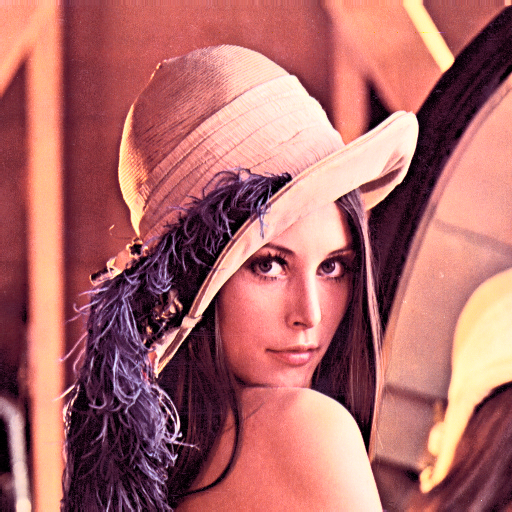
\includegraphics[width=4cm]{Lenna_color_hist.png}
\caption{直方图均衡化}
\label{Lenna:color_hist}
\end{minipage}
\centering
\begin{minipage}[t]{0.30\textwidth}
\centering
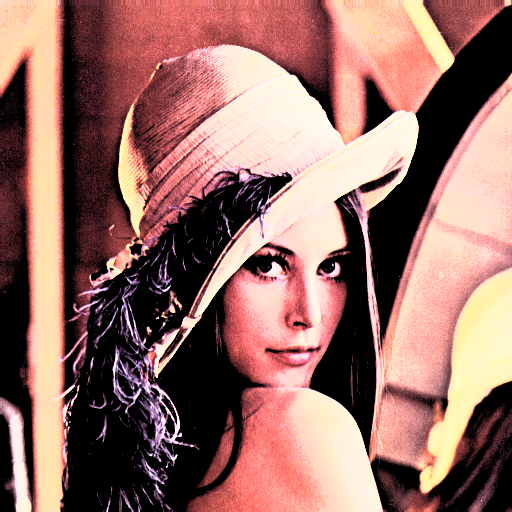
\includegraphics[width=4cm]{Lenna_color_punch_25.png}
\caption{punch纯黑纯白各25\%}
\label{Lenna:color_punch}
\end{minipage}
\centering
\begin{minipage}[t]{0.30\textwidth}
\centering
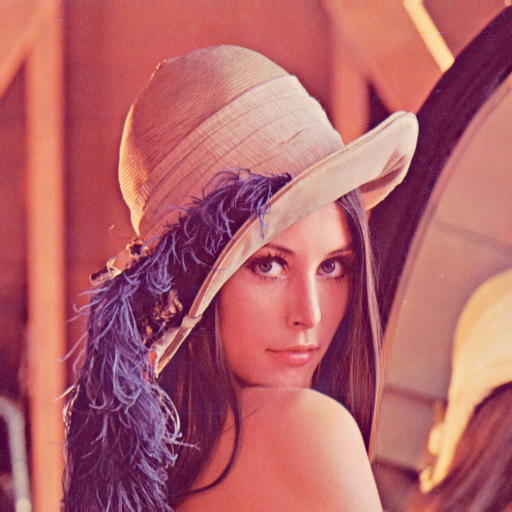
\includegraphics[width=4cm]{Lenna_color_limit_10.png}
\caption{$\lambda=10$}
\label{Lenna:color_lambda}
\end{minipage}
\end{figure}
\end{enumerate}











\subsubsection{night 图片}
\begin{enumerate}[(\romannumeral1)]
	\item 转化为灰度图,转化后见图~\ref{night:gray} :
	\item 原图的直方图见图~\ref{night:count} ,累积分布函数见图~\ref{night:cdf} ,compensation transfer function 为 $f(I)=\alpha×c(I)+(1-\alpha)×I$(局部补偿,见课本公式(3.9)后面),最终直方图均衡化($f(I)=c(I),即\alpha=1$)结果见图~\ref{night:processed},其直方图和累积分布函数分别见图~\ref{night:Pcount} 和图~\ref{night:Pcdf} 。
\begin{figure}[!htbp]
\centering
\begin{minipage}[t]{0.30\textwidth}
\centering
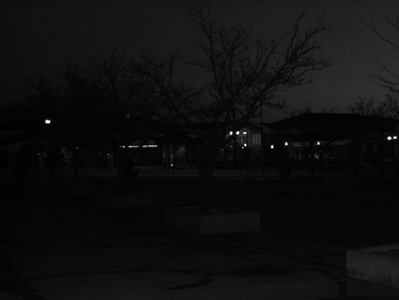
\includegraphics[width=4cm]{night_gray.png}
\caption{night 灰度图}
\label{night:gray}
\end{minipage}
\centering
\begin{minipage}[t]{0.3\textwidth}
\centering
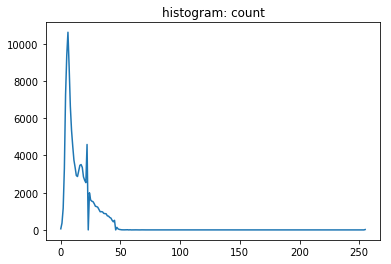
\includegraphics[width=1.0\textwidth]{night_count.png}
\caption{night 直方图}
\label{night:count}
\end{minipage}
\begin{minipage}[t]{0.3\textwidth}
\centering
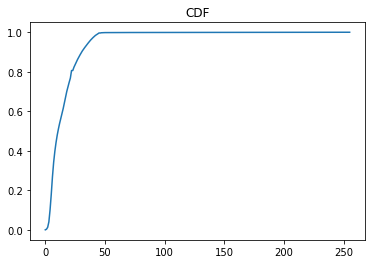
\includegraphics[width=1.0\textwidth]{night_cdf.png}
\caption{累积分布函数}
\label{night:cdf}
\end{minipage}
\centering
\begin{minipage}[t]{0.30\textwidth}
\centering
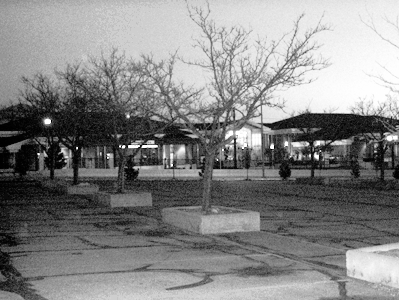
\includegraphics[width=4cm]{night_processed.png}
\caption{night $\alpha=1.00$}
\label{night:processed}
\end{minipage}
\centering
\begin{minipage}[t]{0.3\textwidth}
\centering
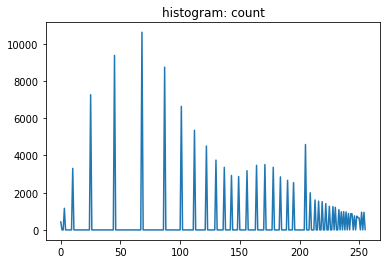
\includegraphics[width=1.0\textwidth]{night_processed_count.png}
\caption{night 直方图}
\label{night:Pcount}
\end{minipage}
\begin{minipage}[t]{0.3\textwidth}
\centering
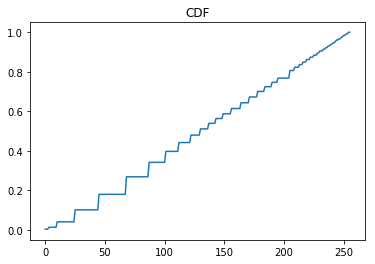
\includegraphics[width=1.0\textwidth]{night_processed_cdf.png}
\caption{累积分布函数}
\label{night:Pcdf}
\end{minipage}
\end{figure}

图~\ref{night:75p} 图~\ref{night:50p} 和图~\ref{night:25p} 分别是$\alpha$分别为0.75,0.5,0.25的图片。\\


\begin{figure}[!htbp]
\centering
\begin{minipage}[t]{0.3\textwidth}
\centering
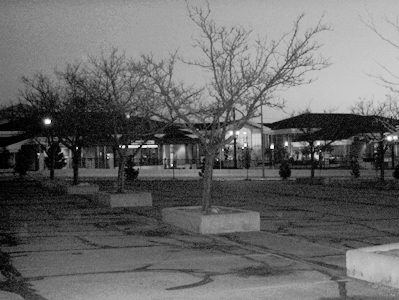
\includegraphics[width=4cm]{night_processed_75.png}
\caption{ $\alpha=0.75$}
\label{night:75p}
\end{minipage}
\begin{minipage}[t]{0.3\textwidth}
\centering
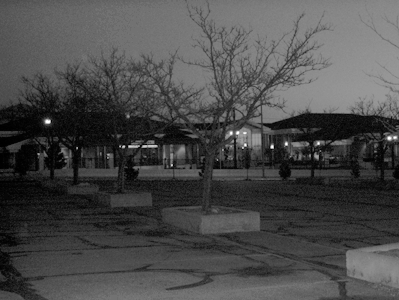
\includegraphics[width=4cm]{night_processed_50.png}
\caption{  $\alpha=0.50$}
\label{night:50p}
\end{minipage}
\begin{minipage}[t]{0.3\textwidth}
\centering
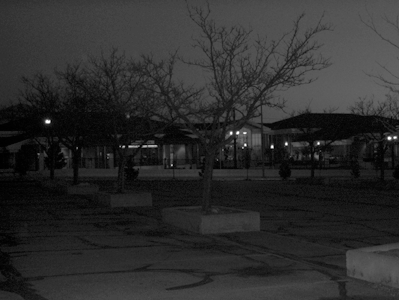
\includegraphics[width=4cm]{night_processed_25.png}
\caption{ $\alpha=0.25$}
\label{night:25p}
\end{minipage}
\end{figure}

	\item punch: punch 纯黑纯白各$5\%, 25\%, 40\%$分别见图~\ref{night:5_punch} 、图~\ref{night:25_punch} 和图~\ref{night:40_punch} 。

\begin{figure}[htbp]
\centering
\begin{minipage}[t]{0.30\textwidth}
\centering
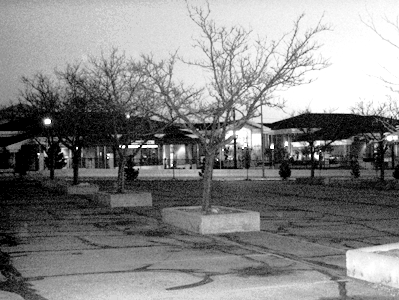
\includegraphics[width=4cm]{night_punch_5.png}
\caption{ punch 5\% - 95\%}
\label{night:5_punch}
\end{minipage}
\centering
\begin{minipage}[t]{0.30\textwidth}
\centering
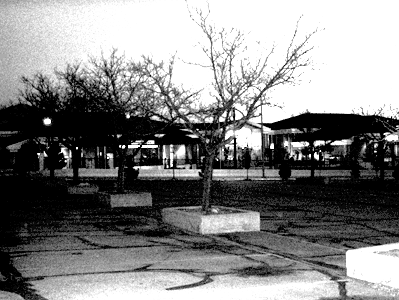
\includegraphics[width=4cm]{night_punch_25.png}
\caption{ punch 25\% - 75\%}
\label{night:25_punch}
\end{minipage}\centering
\begin{minipage}[t]{0.30\textwidth}
\centering
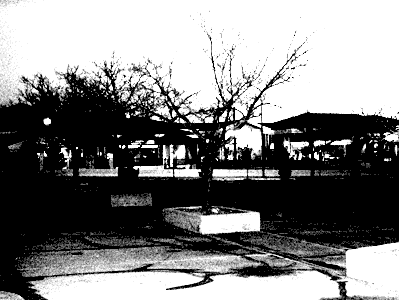
\includegraphics[width=4cm]{night_punch_40.png}
\caption{ punch 40\% - 60\%}
\label{night:40_punch}
\end{minipage}
\end{figure}

	\item limit local gain: 分别将$\lambda N$ 限制在1000, 2000, 5000,见下图:
\begin{figure}[htbp]
\centering
\begin{minipage}[t]{0.30\textwidth}
\centering
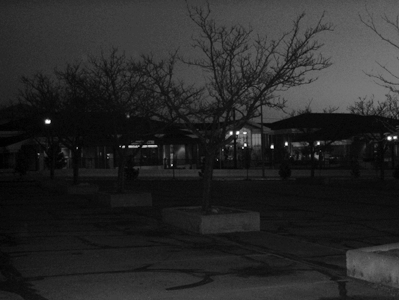
\includegraphics[width=4cm]{night_limit_1000.png}
\caption{$\lambda=1000$}
\label{night:1000_lambda}
\end{minipage}
\centering
\begin{minipage}[t]{0.30\textwidth}
\centering
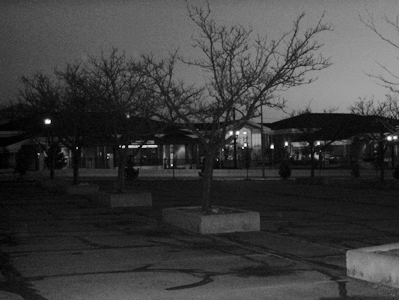
\includegraphics[width=4cm]{night_limit_2000.png}
\caption{$\lambda=2000$}
\label{night:2000_lambda}
\end{minipage}
\centering
\begin{minipage}[t]{0.30\textwidth}
\centering
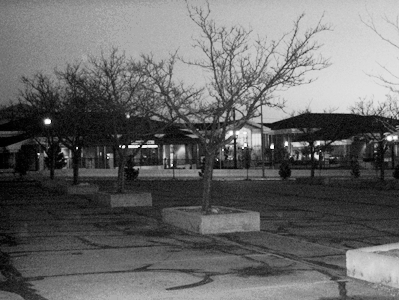
\includegraphics[width=4cm]{night_limit_5000.png}
\caption{$\lambda=5000$}
\label{night:5000_lambda}
\end{minipage}
\end{figure}
	\item gray image to color: 由于是灰色图,不适用
\end{enumerate}





\subsubsection{car 图片}
\begin{enumerate}[(\romannumeral1)]
	\item 转化为灰度图,转化后见图~\ref{car:gray} :
	\item 原图的直方图见图~\ref{car:count} ,累积分布函数见图~\ref{car:cdf}  ,compensation transfer function 为 $f(I)=\alpha×c(I)+(1-\alpha)×I$(局部补偿,见课本公式(3.9)后面),最终直方图均衡化($f(I)=c(I),即\alpha=1$)结果见图~\ref{car:processed},其直方图和累积分布函数分别见图~\ref{car:Pcount} 和图~\ref{car:Pcdf} 。图~\ref{car:75p} 图~\ref{car:50p} 和图~\ref{car:25p} 分别是$\alpha$分别为0.75,0.5,0.25的图片。\\
	\\
	\\
	\\
\begin{figure}[t]
\centering
\begin{minipage}[t]{0.30\textwidth}
\centering
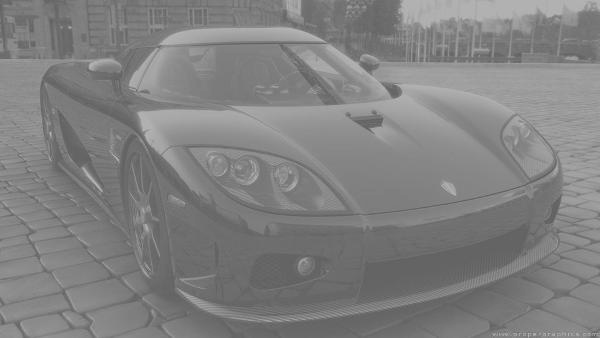
\includegraphics[width=4cm]{car_gray.jpg}
\caption{car 灰度图}
\label{car:gray}
\end{minipage}
\centering
\begin{minipage}[t]{0.3\textwidth}
\centering
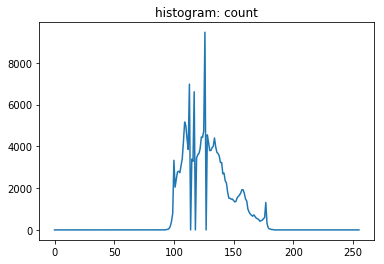
\includegraphics[width=1.0\textwidth]{car_count.png}
\caption{car 直方图}
\label{car:count}
\end{minipage}
\begin{minipage}[t]{0.3\textwidth}
\centering
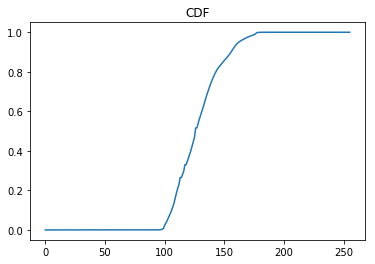
\includegraphics[width=1.0\textwidth]{car_pdf.png}
\caption{累积分布函数}
\label{car:cdf}
\end{minipage}
\centering
\begin{minipage}[t]{0.30\textwidth}
\centering
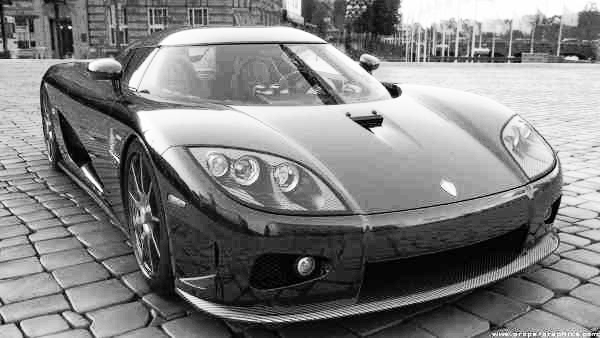
\includegraphics[width=4cm]{car_processed.png}
\caption{car $\alpha=1.00$}
\label{car:processed}
\end{minipage}
\centering
\begin{minipage}[t]{0.3\textwidth}
\centering
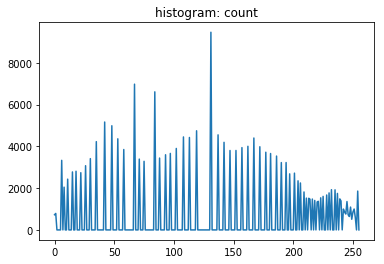
\includegraphics[width=1.0\textwidth]{car_processed_count.png}
\caption{car 直方图}
\label{car:Pcount}
\end{minipage}
\begin{minipage}[t]{0.3\textwidth}
\centering
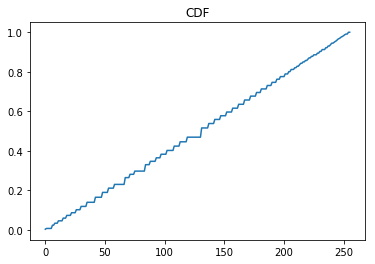
\includegraphics[width=1.0\textwidth]{car_processed_cdf.png}
\caption{累积分布函数}
\label{car:Pcdf}
\end{minipage}
\begin{minipage}[t]{0.3\textwidth}
\centering
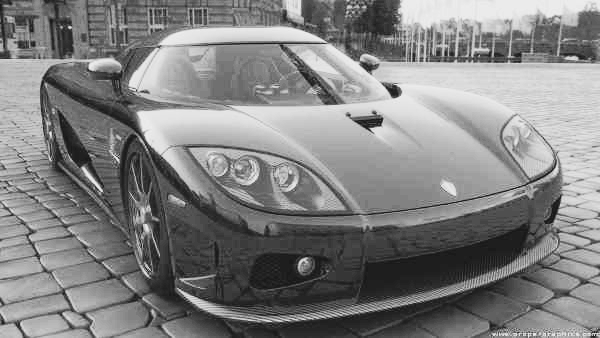
\includegraphics[width=4cm]{car_processed_75.png}
\caption{ $\alpha=0.75$}
\label{car:75p}
\end{minipage}
\begin{minipage}[t]{0.3\textwidth}
\centering
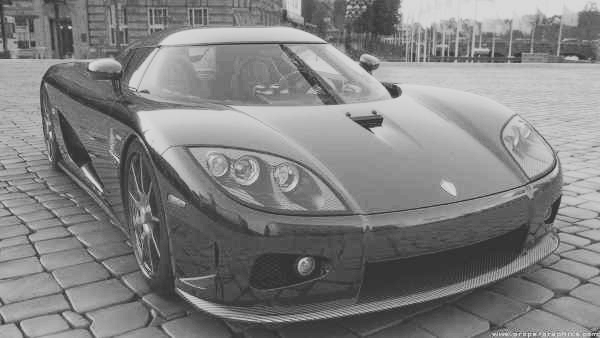
\includegraphics[width=4cm]{car_processed_50.png}
\caption{  $\alpha=0.50$}
\label{car:50p}
\end{minipage}
\begin{minipage}[t]{0.3\textwidth}
\centering
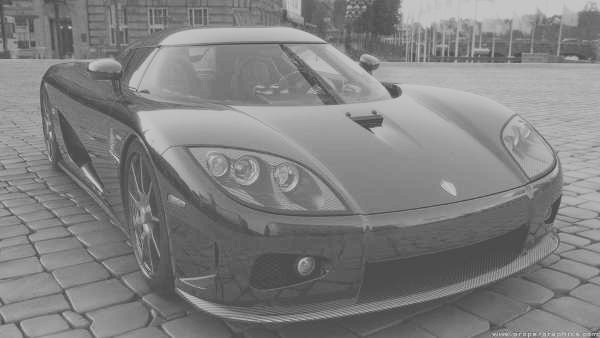
\includegraphics[width=4cm]{car_processed_25.png}
\caption{ $\alpha=0.25$}
\label{car:25p}
\end{minipage}
\end{figure}

	\item punch: punch 纯黑纯白各$5\%, 25\%, 40\%$分别见图~\ref{car:5_punch} 、图~\ref{car:25_punch} 和图~\ref{car:40_punch} 。

\begin{figure}[htbp]
\centering
\begin{minipage}[t]{0.30\textwidth}
\centering
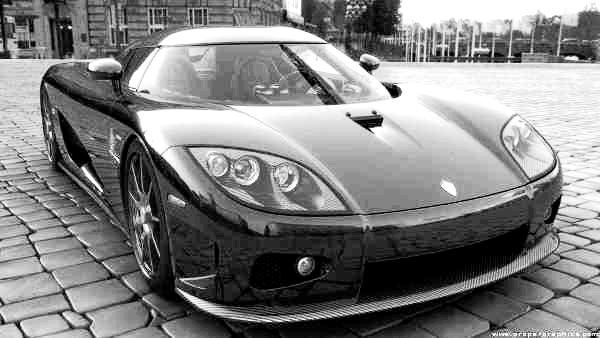
\includegraphics[width=4cm]{car_punch_5.png}
\caption{ punch 5\% - 95\%}
\label{car:5_punch}
\end{minipage}
\centering
\begin{minipage}[t]{0.30\textwidth}
\centering
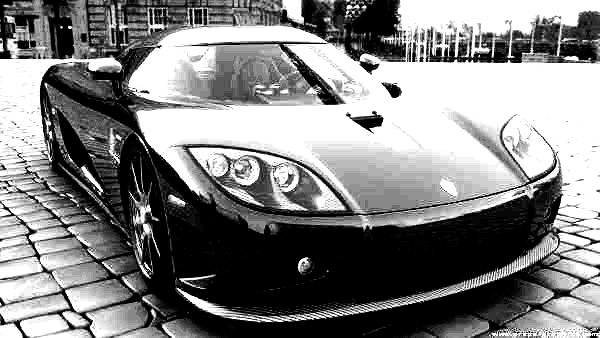
\includegraphics[width=4cm]{car_punch_25.png}
\caption{ punch 25\% - 75\%}
\label{car:25_punch}
\end{minipage}\centering
\begin{minipage}[t]{0.30\textwidth}
\centering
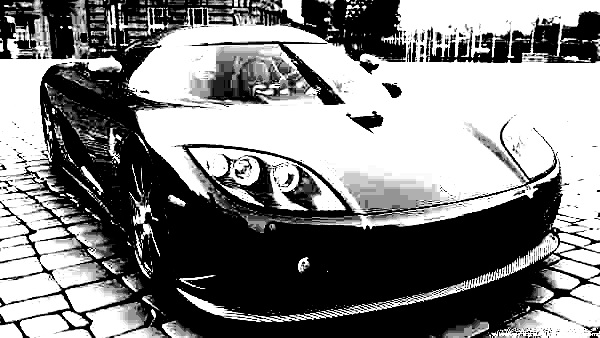
\includegraphics[width=4cm]{car_punch_40.png}
\caption{ punch 40\% - 60\%}
\label{car:40_punch}
\end{minipage}
\end{figure}


	\item limit local gain: 分别将$\lambda$ 限制在100, 1000, 2000,见下图:
\begin{figure}[H]

\begin{minipage}[t]{0.30\textwidth}
\centering
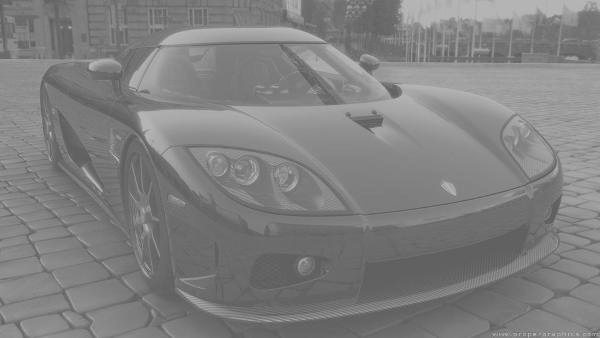
\includegraphics[width=4cm]{car_limit_100.png}
\caption{$\lambda=100$}
\label{car:100_lambda}
\end{minipage}
\centering
\begin{minipage}[t]{0.30\textwidth}
\centering
\includegraphics[width=4cm]{car_limit_1000.png}
\caption{$\lambda=1000$}
\label{car:1000_lambda}
\end{minipage}
\centering
\begin{minipage}[t]{0.30\textwidth}
\centering
\includegraphics[width=4cm]{car_limit_2000.png}
\caption{$\lambda=2000$}
\label{car:2000_lambda}
\end{minipage}
\end{figure}
	\item gray image to color: 由于是灰色图,不适用
\end{enumerate}





\subsection{Local Histogram Equalization}
\qquad 在 Exercise 3.1 基础上,首先将图片转为灰色,对于每个图片分块进行直方图均衡化得到每块的 lookup table,再借助双线性插值法得到每个 pixel 的像素值(不使用低通滤波器)。\par
\begin{enumerate}
	\item 使用 Lenna 图像进行展示,下面分别为 block 为 16*16, 32*32, 64*64得到的局部直方图均衡化图像:
\begin{figure}[H]
\centering
\begin{minipage}[t]{0.30\textwidth}
\centering
\includegraphics[width=4cm]{Lenna_local_16.png}
\caption{$block = 16*16$}
\label{Lenna:16_local}
\end{minipage}
\centering
\begin{minipage}[t]{0.30\textwidth}
\centering
\includegraphics[width=4cm]{Lenna_local_32.png}
\caption{$block = 32*32$}
\label{Lenna:32_local}
\end{minipage}
\centering
\begin{minipage}[t]{0.30\textwidth}
\centering
\includegraphics[width=4cm]{Lenna_local_64.png}
\caption{$block = 64*64$}
\label{Lenna:64_local}
\end{minipage}
\end{figure}
\item 使用 night 图像进行展示,下面分别为 block 为 16*16, 32*32, 64*64得到的局部直方图均衡化图像:
\begin{figure}[H]
\centering
\begin{minipage}[t]{0.30\textwidth}
\centering
\includegraphics[width=4cm]{night_local_16.png}
\caption{$block = 16*16$}
\label{night:16_local}
\end{minipage}
\centering
\begin{minipage}[t]{0.30\textwidth}
\centering
\includegraphics[width=4cm]{night_local_32.png}
\caption{$block = 32*32$}
\label{night:32_local}
\end{minipage}
\centering
\begin{minipage}[t]{0.30\textwidth}
\centering
\includegraphics[width=4cm]{night_local_64.png}
\caption{$block = 64*64$}
\label{night:64_local}
\end{minipage}
\end{figure}
\item 使用 car 图像进行展示,下面分别为 block 为 16*16, 32*32, 64*64得到的局部直方图均衡化图像:
\begin{figure}[H]
\centering
\begin{minipage}[t]{0.30\textwidth}
\centering
\includegraphics[width=4cm]{car_local_16.png}
\caption{$block = 16*16$}
\label{car:16_local}
\end{minipage}
\centering
\begin{minipage}[t]{0.30\textwidth}
\centering
\includegraphics[width=4cm]{car_local_32.png}
\caption{$block = 32*32$}
\label{car:32_local}
\end{minipage}
\centering
\begin{minipage}[t]{0.30\textwidth}
\centering
\includegraphics[width=4cm]{car_local_64.png}
\caption{$block = 64*64$}
\label{car:64_local}
\end{minipage}
\end{figure}
\end{enumerate}






\bibliographystyle{plain}
\bibliography{ref}
\end{document}
